\documentclass[12pt,a4paper]{article}
\usepackage[utf8]{inputenc}
\usepackage[T1]{fontenc}
\usepackage[brazil]{babel}
\usepackage{geometry}
\usepackage{graphicx}
\usepackage{booktabs}
\usepackage{float}
\usepackage{amsmath}
\usepackage{hyperref}
\usepackage{caption}
\usepackage{microtype}

\geometry{left=2.2cm, right=2.2cm, top=2.4cm, bottom=2.4cm}
\setlength{\emergencystretch}{3em}

\title{\textbf{Trabalho Prático 2 -- Simulador de Memória Virtual}\\
\large Sistemas Operacionais -- Departamento de Ciência da Computação (UFMG)}
\author{Aluno 1 \and Davi (Aluno 2)}
\date{Novembro de 2026}

\begin{document}

\maketitle

\section{Introdução}

A gerência de memória virtual por paginação sob demanda permite que processos executem mesmo quando seu espaço de endereçamento excede a memória física disponível, mantendo na RAM apenas as páginas ativas e buscando o restante no armazenamento secundário quando ocorrem faltas de página (\textit{page faults}). O desempenho desse mecanismo depende de duas escolhas fundamentais de projeto no sistema operacional: a estrutura da tabela de páginas, que dita a sobrecarga de memória e o tempo de tradução de endereços, e a política de substituição de páginas, que decide qual quadro físico desalojar quando a memória enche.

Neste trabalho, projetamos e implementamos em linguagem C um simulador de memória virtual parametrizável capaz de processar arquivos de \textit{trace} contendo sequências de referências reais à memória (endereços hexadecimais de 32 bits acompanhados da operação de leitura \texttt{R} ou escrita \texttt{W}). O simulador foi construído em quatro módulos principais: o ponto de entrada (\texttt{main.c}), responsável pela leitura dos parâmetros e geração do relatório de saída; o núcleo da unidade de gerenciamento de memória (\texttt{mmu.c}), que coordena o ciclo de tradução, controle de bits de estado e contabilização de leituras e escritas em disco; o módulo de estruturas de tradução (\texttt{pagetable.c}), contendo quatro organizações de tabela de páginas; e o módulo de políticas de substituição (\texttt{algoritmos.c}).

Além de avaliar os quatro programas de referência (\texttt{compilador.log}, \texttt{compressor.log}, \texttt{matriz.log} e \texttt{simulador.log}) sob crescimento da memória física (128 KB a 16 MB) e variação do tamanho de página (2 KB a 64 KB), estendemos a investigação experimental em três frentes adicionais:
\begin{enumerate}
    \item A inclusão do \textbf{Algoritmo Ótimo Teórico de Belady (\texttt{opt})} como limite inferior matemático de faltas de página nos gráficos comparativos;
    \item Um estudo em escala da \textbf{Anomalia de Belady}, avaliando a frequência com que o aumento de quadros físicos degrada o desempenho em políticas de fila (FIFO e CLOCK) frente à imunidade dos algoritmos de pilha (LRU e Ótimo) conforme variamos o número de quadros e o tamanho da entrada;
    \item Uma análise do impacto do \textbf{\textit{dirty bit} (bit de modificação)}, contrastando o volume real de escritas em disco contra um cenário hipotético sem verificação de \textit{dirty bit} (no qual 100\% das páginas substituídas exigem escrita em disco) para comparar o comportamento do LRU e do CLOCK diante de páginas modificadas.
\end{enumerate}

\section{Motivação e Metodologia de Implementação}

\subsection{Metodologia Geral da MMU}

A unidade de gerenciamento de memória (\texttt{MMU}) divide a memória física total em $Q = \text{tam\_memoria\_KB} / \text{tam\_pagina\_KB}$ quadros físicos. Como o tamanho de página pode variar entre potências de 2 (de 2 KB a 64 KB), o número de bits de deslocamento interno ($s$) é derivado na inicialização deslocando-se o tamanho da página em bytes para a direita até atingir $1$, de modo que $s = \log_2(\text{tam\_pagina\_bytes})$. Assim, para cada endereço de 32 bits lido do arquivo, o número da página virtual (VPN) é obtido por \texttt{vpn = addr >> s}, restando $b = 32 - s$ bits significativos para identificação da página.

A cada acesso processado, a MMU consulta a tabela de páginas pelo \texttt{vpn}. Caso a página já esteja residente em um quadro físico (\textit{page hit}), atualiza-se o bit de referência daquele quadro para $1$, registra-se o instante atual do contador global de acessos e, se a operação for \texttt{W}, marca-se o bit de modificação (\textit{dirty}). Caso a página não esteja mapeada (\textit{page fault}), contabiliza-se uma página lida. Enquanto houver quadros livres, eles são ocupados sequencialmente; quando todos os $Q$ quadros estão cheios, o algoritmo de substituição seleciona um quadro vítima. Se o quadro vítima estiver marcado como modificado (\textit{dirty}), contabiliza-se uma página escrita em disco antes de invalidar seu mapeamento antigo e carregar a nova página.

\subsection{Algoritmos de Substituição de Páginas}

Selecionamos quatro políticas práticas que cobrem os critérios do enunciado e adicionamos o algoritmo Ótimo para referência teórica:

\begin{itemize}
    \item \textbf{Random (Aleatoriedade):}
    \begin{itemize}
        \item \textit{Motivação:} Serve como linha de base estocástica de custo $O(1)$. Permite verificar em que medida algoritmos que mantêm histórico superam uma escolha cega e observar casos patológicos em que o sorteio evita sincronizações cíclicas.
        \item \textit{Metodologia de implementação:} Utiliza o gerador pseudoaleatório padrão do C inicializado com semente fixa (\texttt{srandom(42)}) e seleciona o índice do quadro vítima por aritmética modular direta sobre o total de quadros (\texttt{random() \% num\_quadros}).
    \end{itemize}

    \item \textbf{LRU -- Least Recently Used (Histórico de Acessos Recentes):}
    \begin{itemize}
        \item \textit{Motivação:} Explora diretamente a localidade temporal sob a premissa de que páginas referenciadas há menos tempo têm maior chance de reuso imediato.
        \item \textit{Metodologia de implementação:} Foi implementado pelo método de contador lógico de tempo. A MMU mantém um contador global incrementado a cada referência à memória; todo acesso a um quadro (seja carga ou \textit{hit}) copia o valor atual desse contador para o carimbo de último acesso do quadro. Na falta de página, a função de substituição realiza uma busca linear $O(Q)$ sobre o vetor de quadros físicos e seleciona aquele que possui o menor carimbo de tempo.
    \end{itemize}

    \item \textbf{CLOCK / Segunda Chance (Frequência e Uso Recente):}
    \begin{itemize}
        \item \textit{Motivação:} Aproximar o comportamento do LRU utilizando apenas 1 bit de referência por página, eliminando a necessidade de atualizar carimbos de 64 bits a cada acesso e de varrer todos os quadros em toda substituição.
        \item \textit{Metodologia de implementação:} Organiza o vetor de quadros como uma lista circular percorrida por um ponteiro persistente. Quando uma vítima é necessária, o algoritmo inspeciona o quadro atual: se o bit de referência estiver ativo ($1$), o quadro recebe uma segunda chance (seu bit é zerado para $0$ e o ponteiro avança circularmente); o laço prossegue até encontrar o primeiro quadro com bit de referência igual a $0$, que é retornado como vítima, deixando o ponteiro posicionado no quadro imediatamente seguinte para a próxima chamada.
    \end{itemize}

    \item \textbf{FIFO -- First-In, First-Out (Critério Livre):}
    \begin{itemize}
        \item \textit{Motivação:} Avaliar o impacto de substituir páginas puramente pela idade de carregamento na memória, ignorando sua frequência de leitura ou escrita, além de permitir a reprodução experimental da Anomalia de Belady.
        \item \textit{Metodologia de implementação:} Como os quadros livres são preenchidos em ordem estritamente sequencial no início da simulação, a fila FIFO é implementada de forma exata em $O(1)$ por meio de um único ponteiro circular de substituição: a cada falta com memória cheia, o quadro apontado (o mais antigo presente na RAM) é escolhido como vítima e o ponteiro avança em módulo $Q$.
    \end{itemize}

    \item \textbf{Ótimo de Belady -- \texttt{opt} (Referência Teórica):}
    \begin{itemize}
        \item \textit{Motivação:} Estabelecer o limite inferior absoluto de faltas de página que qualquer política de substituição poderia atingir para um dado arquivo de entrada e tamanho de memória.
        \item \textit{Metodologia de implementação:} Como o algoritmo ótimo requer conhecer o futuro, sua execução realiza um pré-processamento linear $O(N)$ em duas passagens sobre o \textit{trace}. Primeiro, a sequência de $N$ acessos é carregada em memória; em seguida, percorrendo o vetor de trás para frente (do índice $N-1$ até $0$) com o auxílio de uma tabela auxiliar da última aparição vista de cada VPN, anota-se para cada acesso $i$ o índice exato de sua próxima referência futura (ou $\infty$, representado por \texttt{ULONG\_MAX}, caso a página não volte a ser usada). Durante a simulação, cada quadro armazena o índice do próximo acesso de sua página atual, e a substituição escolhe o quadro com o maior valor (o uso mais distante no futuro).
    \end{itemize}
\end{itemize}

\subsection{Estruturas de Tabela de Páginas}

Para investigar o compromisso entre consumo de memória e velocidade de consulta na tradução de endereços de 32 bits ($b = 32 - s$ bits de VPN), implementamos as quatro arquiteturas exigidas:

\begin{enumerate}
    \item \textbf{Tabela Densa (1 Nível):} Implementada como um único vetor contíguo de $2^b$ inteiros alocado integralmente na inicialização e inicializado com $-1$ (página ausente). A busca, o mapeamento e o desmapeamento consistem em indexação direta pelo próprio \texttt{vpn} em $O(1)$.
    \item \textbf{Tabela Hierárquica de 2 Níveis:} Divide os $b$ bits do VPN em duas metades: $b_1 = \lfloor b/2 \rfloor$ bits superiores para indexar o diretório de nível 1 e $b_2 = b - b_1$ bits inferiores para a tabela de nível 2 (para páginas de 4 KB, $10 + 10$ bits). Inicialmente, apenas o vetor de ponteiros de nível 1 é alocado com \texttt{calloc}. As sub-tabelas de nível 2 são alocadas sob demanda via \texttt{malloc} apenas quando uma página pertencente àquela entrada do diretório é mapeada pela primeira vez.
    \item \textbf{Tabela Hierárquica de 3 Níveis:} Particiona os $b$ bits do VPN em três fatias ($b_1 = \lfloor b/3 \rfloor$, $b_2 = \lfloor b/3 \rfloor$ e $b_3 = b - b_1 - b_2$, resultando em $6 + 6 + 8$ bits para páginas de 4 KB). A tradução realiza três extrações por máscara de bits e deslocamento, alocando diretórios intermediários (nível 2) e tabelas folhas (nível 3) estritamente sob demanda.
    \item \textbf{Tabela Invertida:} Dimensionada pelo número de quadros físicos $Q$ (e não pelo espaço virtual $2^b$). Foi implementada como uma tabela hash com encadeamento estático em vetor: um arranjo de cabeças de lista de tamanho $Q$ e um arranjo paralelo de $Q$ nós (um por quadro físico), onde cada nó guarda o \texttt{vpn} atualmente armazenado naquele quadro e o índice do próximo quadro na mesma lista de colisão. A função de dispersão multiplica o VPN pela constante áurea de Knuth ($\text{vpn} \times 2654435761 \bmod Q$), garantindo busca em tempo médio $O(1)$ e ocupação de memória proporcional apenas à RAM física.
\end{enumerate}

\section{Decisões de Projeto}

Durante o desenvolvimento do simulador e da bateria experimental, adotamos as seguintes decisões de projeto:
\begin{enumerate}
    \item \textbf{Implementação separada do Algoritmo Ótimo (\texttt{opt}):} A decisão de implementar o algoritmo Ótimo surgiu após a conclusão dos quatro algoritmos principais, quando analisávamos os primeiros gráficos e sentimos necessidade de um referencial teórico para avaliar quão próximos o LRU e o CLOCK estavam do melhor resultado matematicamente possível. Como o Ótimo exige pré-carregar toda a sequência futura de acessos (ao contrário das políticas reais que operam em \textit{streaming} linha a linha), isolamos sua rotina de pré-processamento na execução do arquivo: quando o simulador é chamado com \texttt{lru}, \texttt{clock}, \texttt{fifo} ou \texttt{random}, ele mantém o loop original de leitura direta sem alocar vetores de futuro; o pré-carregamento só é ativado quando o argumento \texttt{opt} é solicitado para fins de comparação nos gráficos.
    \item \textbf{Seleção de tabela de páginas via 5º argumento opcional:} Para preservar total compatibilidade com a chamada padrão de 4 argumentos especificada no enunciado (\texttt{./simulador <alg> <arq> <pag> <mem>}), a tabela densa é adotada por padrão quando apenas 4 parâmetros são passados. Quando um quinto argumento opcional é informado (\texttt{densa}, \texttt{hier2}, \texttt{hier3} ou \texttt{invertida}), o simulador instancia a tabela correspondente e imprime uma linha adicional informando o total exato de bytes alocados pela estrutura.
    \item \textbf{Regra de escrita de páginas sujas:} Seguindo estritamente o enunciado, páginas com \textit{dirty bit} ativo somente geram escrita em disco no instante em que são escolhidas como vítimas e substituídas. Páginas modificadas que permanecem residentes na memória ao final da simulação não são contabilizadas como escritas.
\end{enumerate}

\section{Análise de Desempenho}

\subsection{Cenário 1: Crescimento da Memória Física (Páginas de 4 KB)}

Neste primeiro cenário, fixamos o tamanho da página em 4 KB e variamos a memória física disponível em potências de 2, de 128 KB (32 quadros) até 16384 KB (4096 quadros). A Figura~\ref{fig:cenario1} apresenta as curvas de faltas de página incluindo o limite teórico \textbf{Ótimo (\texttt{OPT})}, e a Tabela~\ref{tab:cenario1} resume os valores de páginas lidas e escritas.

\begin{figure}[H]
    \centering
    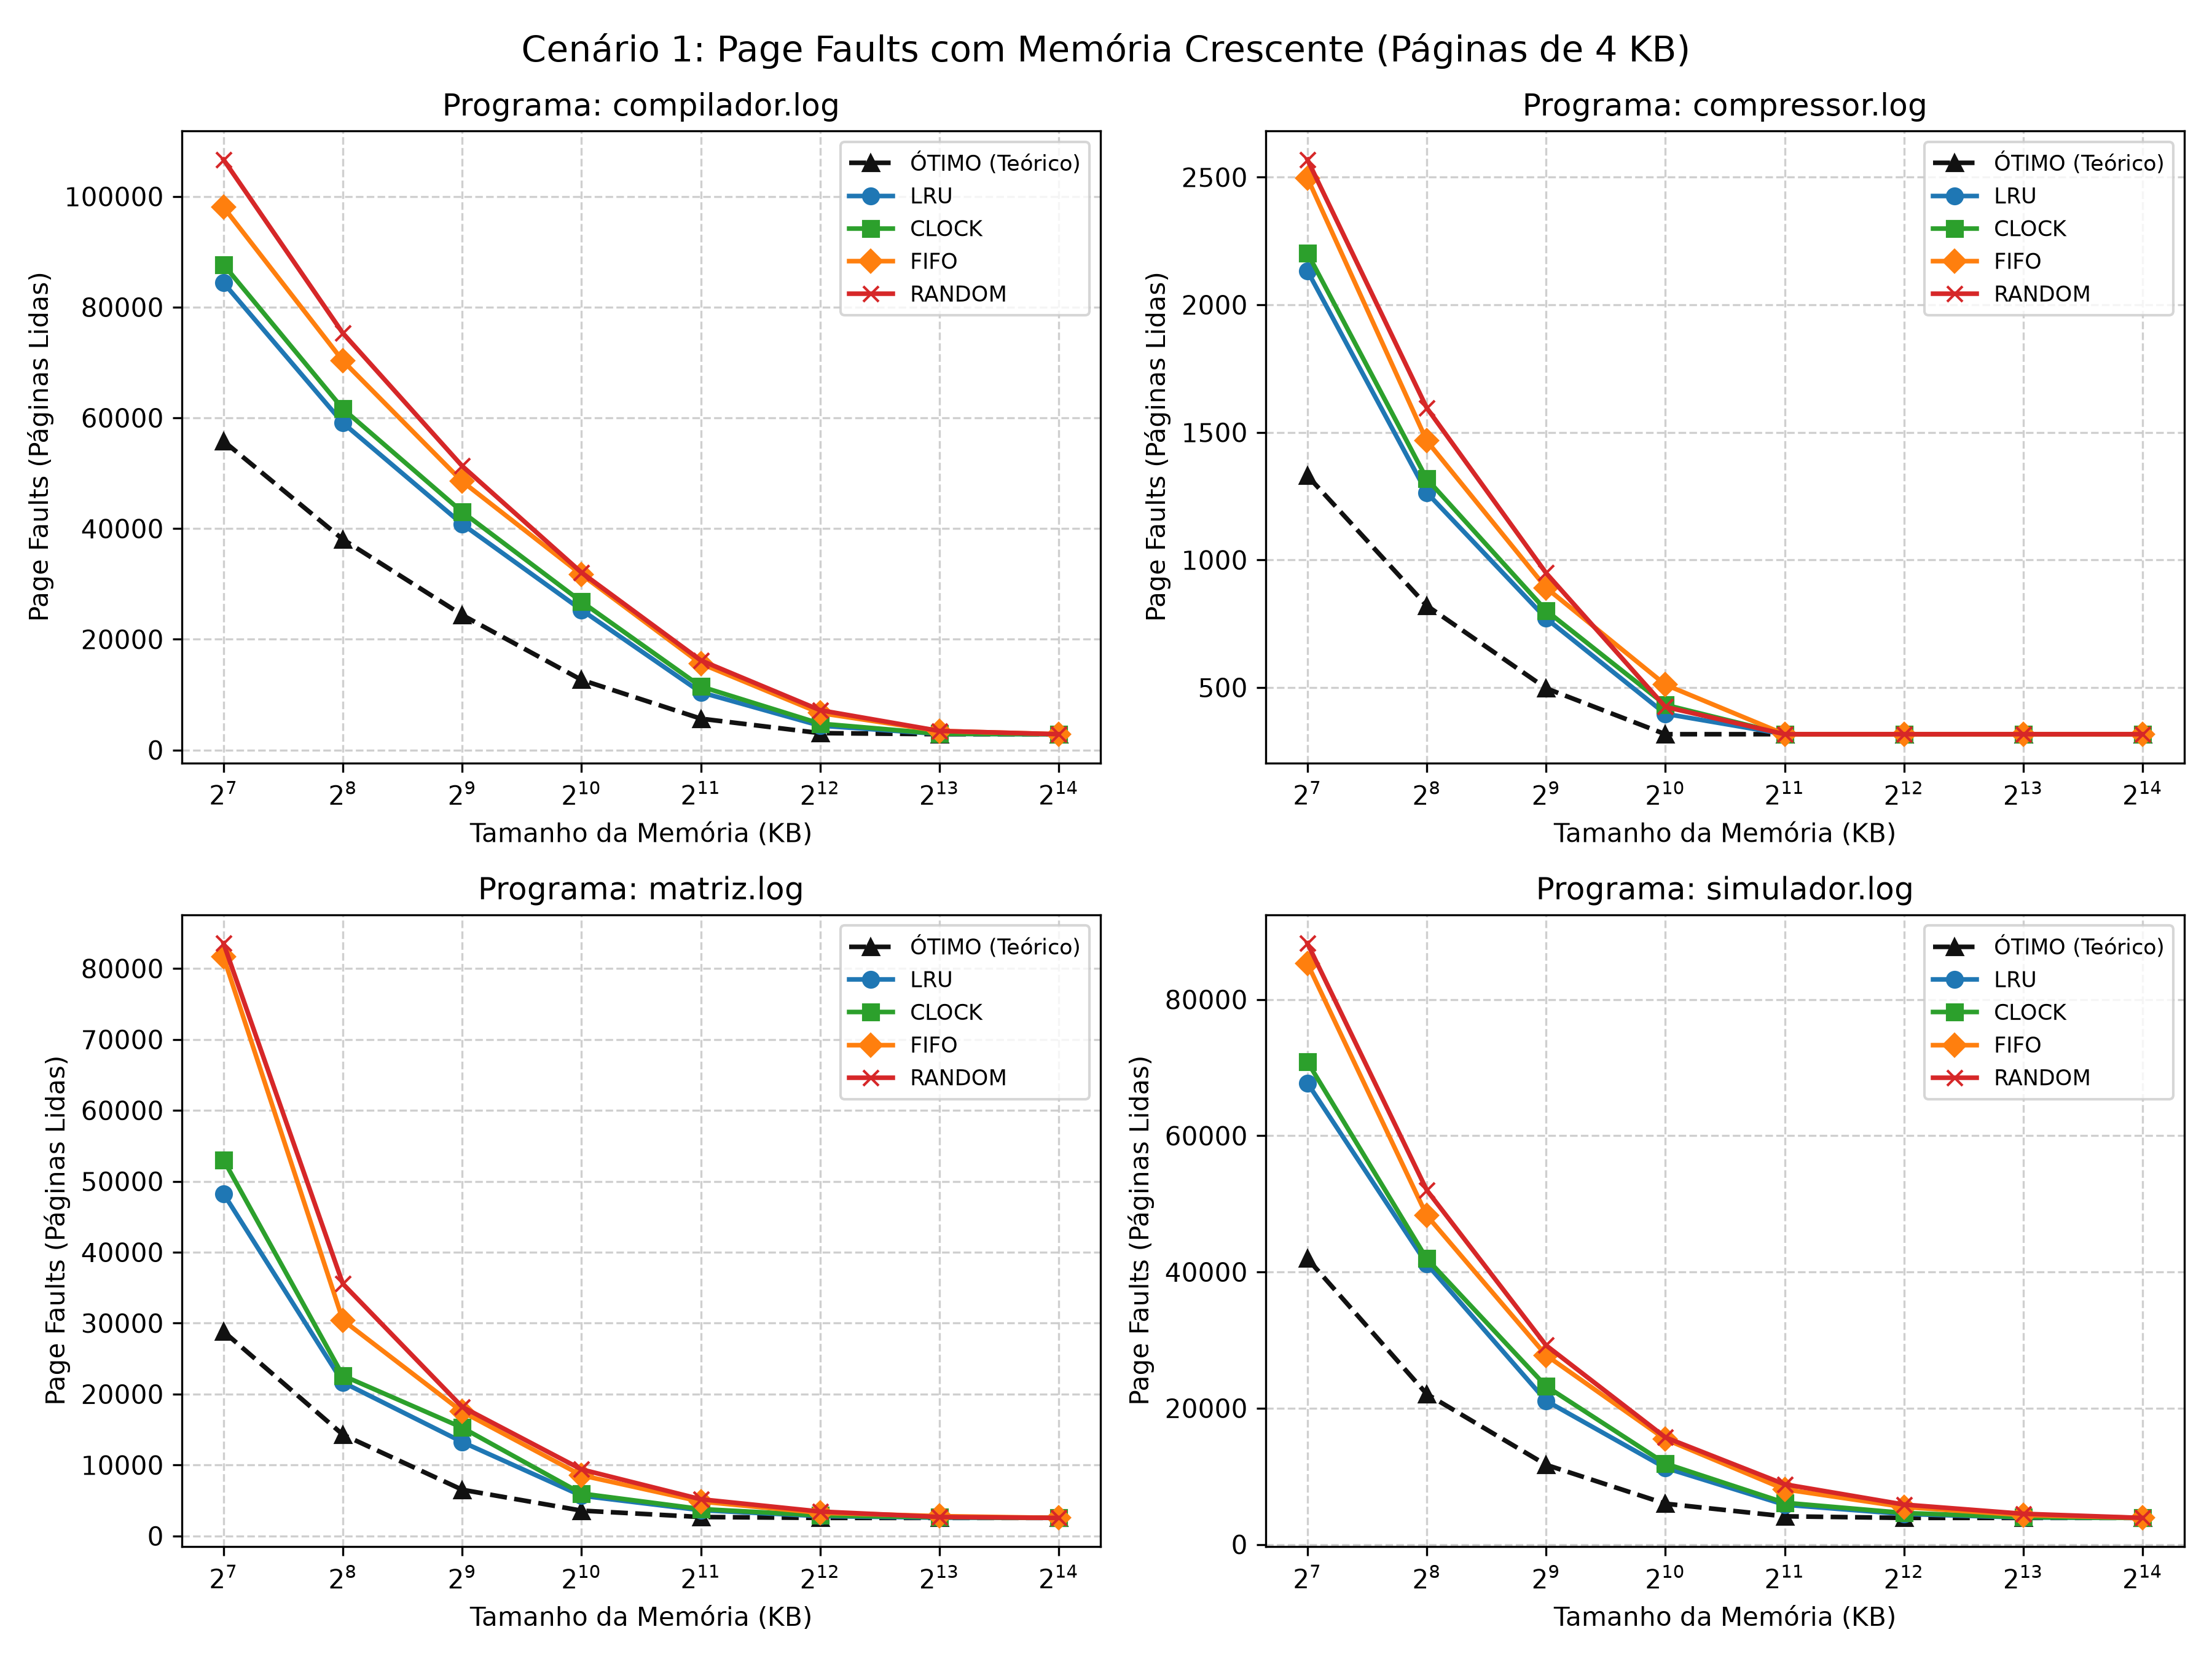
\includegraphics[width=1.0\textwidth]{results/cenario1_page_faults.png}
    \caption{Faltas de página em função do tamanho da memória física com páginas fixas de 4 KB (incluindo o limite teórico Ótimo).}
    \label{fig:cenario1}
\end{figure}

\begin{table}[H]
\centering
\caption{Páginas lidas (faltas) e páginas escritas no Cenário 1 (páginas de 4 KB).}
\label{tab:cenario1}
\resizebox{\textwidth}{!}{%
\begin{tabular}{llrrrrr}
\toprule
\textbf{Programa} & \textbf{Memória} & \textbf{ÓTIMO (L / E)} & \textbf{LRU (L / E)} & \textbf{CLOCK (L / E)} & \textbf{FIFO (L / E)} & \textbf{Random (L / E)} \\
\midrule
\texttt{compilador.log} & 128 KB   & 55.802 / 8.274  & 84.401 / 11.737 & 87.686 / 12.293 & 98.067 / 16.759 & 106.655 / 17.065 \\
                        & 512 KB   & 24.391 / 3.968  & 40.821 / 6.131  & 43.017 / 6.671  & 48.526 / 8.487  & 51.306 / 8.575   \\
                        & 2048 KB  & 5.662 / 1.328   & 10.425 / 2.173  & 11.472 / 2.398  & 15.609 / 3.425  & 16.190 / 3.384   \\
                        & 16384 KB & 2.852 / 0       & 2.852 / 0       & 2.852 / 0       & 2.852 / 0       & 2.852 / 0        \\
\midrule
\texttt{compressor.log} & 128 KB   & 1.330 / 460     & 2.133 / 702     & 2.203 / 734     & 2.497 / 851     & 2.569 / 849      \\
                        & 512 KB   & 497 / 137       & 771 / 224       & 802 / 235       & 891 / 305       & 949 / 321        \\
                        & 2048 KB  & 317 / 0         & 317 / 0         & 317 / 0         & 317 / 0         & 317 / 0          \\
                        & 16384 KB & 317 / 0         & 317 / 0         & 317 / 0         & 317 / 0         & 317 / 0          \\
\midrule
\texttt{matriz.log}     & 128 KB   & 28.826 / 6.910  & 48.254 / 9.674  & 53.025 / 11.140 & 81.638 / 18.172 & 83.549 / 18.345  \\
                        & 512 KB   & 6.518 / 2.134   & 13.250 / 3.812  & 15.275 / 4.371  & 17.523 / 4.932  & 18.199 / 5.100   \\
                        & 2048 KB  & 2.672 / 985     & 3.632 / 1.159   & 3.795 / 1.218   & 4.850 / 1.624   & 5.174 / 1.747    \\
                        & 16384 KB & 2.543 / 0       & 2.543 / 0       & 2.543 / 0       & 2.543 / 0       & 2.543 / 0        \\
\midrule
\texttt{simulador.log}  & 128 KB   & 41.955 / 10.023 & 67.747 / 13.730 & 70.849 / 14.432 & 85.283 / 18.805 & 88.247 / 19.479  \\
                        & 512 KB   & 11.690 / 4.129  & 21.090 / 6.526  & 23.229 / 7.226  & 27.778 / 8.346  & 29.231 / 8.508   \\
                        & 2048 KB  & 4.125 / 1.884   & 5.823 / 2.444   & 6.119 / 2.587   & 8.089 / 3.353   & 8.826 / 3.494    \\
                        & 16384 KB & 3.890 / 0       & 3.890 / 0       & 3.890 / 0       & 3.890 / 0       & 3.890 / 0        \\
\bottomrule
\end{tabular}%
}
\end{table}

Os resultados permitem extrair três conclusões principais:
\begin{enumerate}
    \item \textbf{Desempenho de CLOCK e LRU frente ao Limite Ótimo:} Em todos os programas e tamanhos de memória, as curvas de \texttt{lru} (azul) e \texttt{clock} (verde) permanecem praticamente coladas. No \texttt{compilador.log} com 128 KB, o CLOCK apresenta apenas $3,9\%$ mais faltas que o LRU ($87.686$ contra $84.401$). O algoritmo \texttt{opt} (curva tracejada preta) estabelece o piso teórico em $55.802$ faltas, evidenciando que o uso de 1 único bit de referência no CLOCK recupera quase toda a vantagem que o LRU obtém sobre o Random ($106.655$ faltas).
    \item \textbf{Degradação severa do FIFO e do Random em loops matriciais:} A maior distância entre as políticas práticas ocorre em \texttt{matriz.log} sob memória restrita (128 KB). Enquanto o LRU gera $48.254$ faltas ($9.674$ escritas) e o CLOCK gera $53.025$ faltas ($11.140$ escritas), o FIFO salta para $81.638$ faltas e $18.172$ escritas ($69\%$ a mais de faltas e quase o dobro de escritas em disco). Em operações matriciais, blocos de linhas e variáveis acumuladoras são lidos e modificados repetidamente; como foram carregados no início da execução, o FIFO os elege como vítimas justamente enquanto ainda estão em uso ativo.
    \item \textbf{Convergência e tamanho do Conjunto de Trabalho (\textit{Working Set}):} À medida que a memória cresce, todas as 5 curvas convergem para o mesmo piso de faltas compulsórias (\textit{cold misses}) quando o conjunto de trabalho passa a caber inteiro na RAM. No \texttt{compressor.log}, o conjunto de trabalho total é de apenas $317$ páginas de 4 KB ($\approx 1,24\text{ MB}$), estabilizando a partir de 2048 KB (e no \texttt{opt} já em 1024 KB com $317$ leituras). Nos demais programas, a convergência completa ocorre em 16384 KB ($2.852$ páginas únicas no \texttt{compilador}, $2.543$ na \texttt{matriz} e $3.890$ no \texttt{simulador}).
\end{enumerate}

\subsection{Cenário 2: Variação do Tamanho de Página (Memória Fixa em 1024 KB)}

No segundo experimento, mantivemos a memória física fixa em 1024 KB e variamos o tamanho da página de 2 KB a 64 KB. Com memória total constante, dobrar o tamanho da página reduz pela metade a quantidade de quadros físicos disponíveis: de $512$ quadros (em 2 KB) para apenas $16$ quadros (em 64 KB). A Figura~\ref{fig:cenario2} e a Tabela~\ref{tab:cenario2} apresentam os resultados.

\begin{figure}[H]
    \centering
    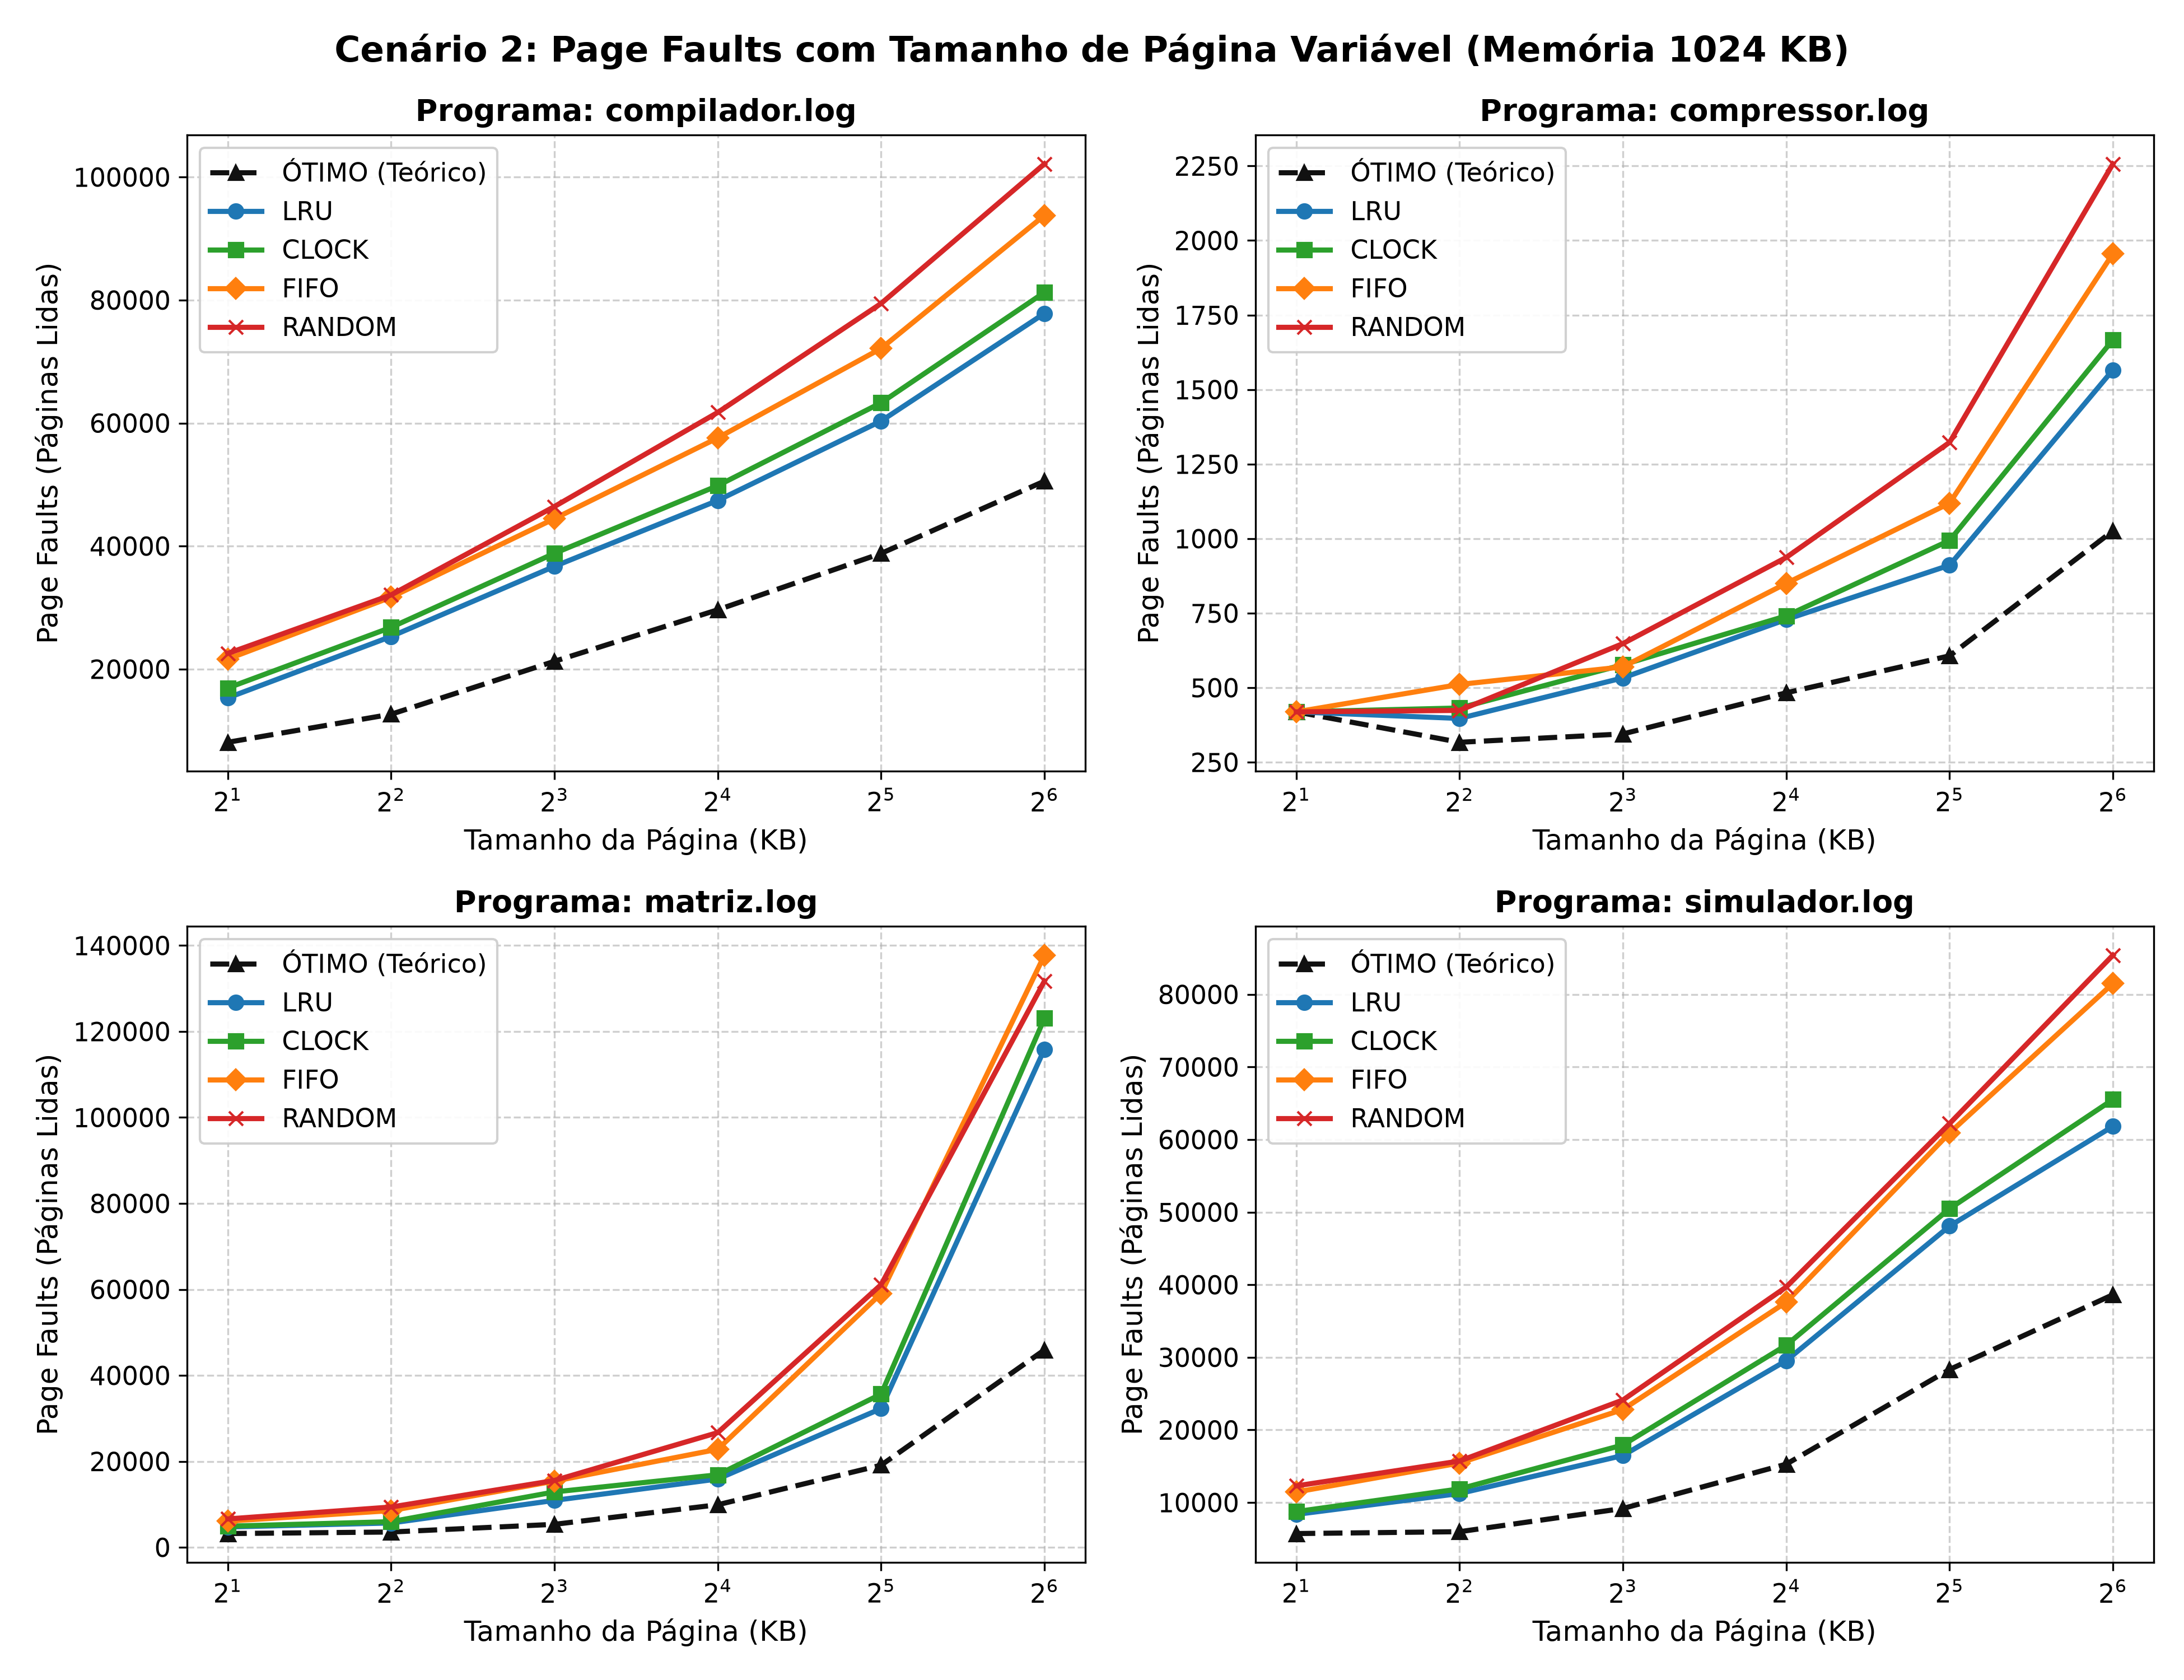
\includegraphics[width=1.0\textwidth]{results/cenario2_page_faults.png}
    \caption{Faltas de página com memória fixa em 1024 KB e tamanho de página variando de 2 KB a 64 KB.}
    \label{fig:cenario2}
\end{figure}

\begin{table}[H]
\centering
\caption{Faltas de página (páginas lidas) no Cenário 2 com memória física fixa de 1024 KB.}
\label{tab:cenario2}
\resizebox{\textwidth}{!}{%
\begin{tabular}{llrrrrrr}
\toprule
\textbf{Programa} & \textbf{Algoritmo} & \textbf{2 KB (512 q.)} & \textbf{4 KB (256 q.)} & \textbf{8 KB (128 q.)} & \textbf{16 KB (64 q.)} & \textbf{32 KB (32 q.)} & \textbf{64 KB (16 q.)} \\
\midrule
\texttt{compilador.log} & ÓTIMO  & 7.835  & 12.667 & 19.345 & 26.866 & 36.221 & 48.613  \\
                        & LRU    & 15.330 & 25.308 & 36.707 & 47.424 & 60.336 & 77.837  \\
                        & CLOCK  & 16.936 & 26.789 & 38.827 & 49.831 & 63.302 & 81.255  \\
                        & FIFO   & 21.639 & 31.698 & 44.465 & 57.600 & 72.140 & 93.778  \\
                        & Random & 22.550 & 32.062 & 46.435 & 61.738 & 79.448 & 102.142 \\
\midrule
\texttt{compressor.log} & ÓTIMO  & 419    & \textbf{317} & 346 & 424   & 567    & 961     \\
                        & LRU    & 419    & \textbf{397} & 533 & 729   & 911    & 1.566   \\
                        & CLOCK  & 419    & 432    & 577    & 741    & 994    & 1.667   \\
                        & FIFO   & 419    & 511    & 570    & 850    & 1.119  & 1.956   \\
                        & Random & 419    & 424    & 648    & 937    & 1.323  & 2.257   \\
\midrule
\texttt{matriz.log}     & ÓTIMO  & 3.631  & 3.572  & 5.158  & 9.217  & 20.514 & 61.675  \\
                        & LRU    & 4.744  & 5.673  & 10.928 & 15.904 & 32.282 & 115.886 \\
                        & CLOCK  & 4.924  & 5.980  & 12.896 & 16.884 & 35.656 & 123.055 \\
                        & FIFO   & 6.097  & 8.551  & 15.410 & 22.815 & 59.061 & 137.751 \\
                        & Random & 6.613  & 9.384  & 15.560 & 26.696 & 61.112 & \textbf{131.729} \\
\midrule
\texttt{simulador.log}  & ÓTIMO  & 5.922  & 5.981  & 8.854  & 15.655 & 26.471 & 38.685  \\
                        & LRU    & 8.364  & 11.240 & 16.479 & 29.547 & 48.088 & 61.829  \\
                        & CLOCK  & 8.749  & 11.876 & 17.923 & 31.677 & 50.484 & 65.522  \\
                        & FIFO   & 11.449 & 15.440 & 22.816 & 37.606 & 60.922 & 81.506  \\
                        & Random & 12.290 & 15.715 & 24.125 & 39.697 & 62.207 & 85.408  \\
\bottomrule
\end{tabular}%
}
\end{table}

A variação do tamanho de página evidencia o compromisso entre \textbf{localidade espacial} e \textbf{fragmentação interna / escassez de quadros}:
\begin{enumerate}
    \item \textbf{Aproveitamento de localidade espacial de 2 KB para 4 KB:} Na passagem de 2 KB para 4 KB no \texttt{compressor.log}, o número de faltas \textit{cai} de $419$ para $397$ no LRU e de $419$ para $317$ no Ótimo (e no \texttt{matriz.log} com Ótimo cai de $3.631$ para $3.572$). Quando a página dobra de 2 KB para 4 KB, cada leitura carrega endereços vizinhos contíguos que são acessados logo em seguida.
    \item \textbf{Degradação por redução do número de quadros e fragmentação interna:} A partir de 8 KB (e de forma crítica em 32 KB e 64 KB), o número de faltas cresce acentuadamente em todos os programas. Com páginas de 64 KB, a memória de 1024 KB possui apenas \textbf{16 quadros físicos}. No \texttt{compilador.log}, que realiza acessos espalhados em árvores sintáticas e tabelas de símbolos, carregar blocos de 64 KB traz grande quantidade de bytes que não serão utilizados (fragmentação interna) e reduz o número de regiões distintas que podem coexistir na RAM, quintuplicando as faltas no LRU (de $15.330$ em 2 KB para $77.837$ em 64 KB).
    \item \textbf{Colapso em \texttt{matriz.log} com 64 KB e inversão entre FIFO e Random:} No \texttt{matriz.log}, passar de 32 KB (32 quadros) para 64 KB (16 quadros) faz as faltas no LRU saltarem quase quatro vezes (de $32.282$ para $115.886$). Isso indica que o laço interno do cálculo matricial toca simultaneamente em mais de 16 faixas de 64 KB, causando \textit{thrashing}. Nesse ponto extremo (64 KB), observa-se inclusive que o \textbf{Random} ($131.729$ faltas) supera o \textbf{FIFO} ($137.751$ faltas): quando um percurso cíclico sobre matrizes excede a capacidade da fila do FIFO, ele substitui sistematicamente a página que será pedida na próxima iteração, enquanto a escolha aleatória quebra essa sincronização destrutiva.
\end{enumerate}

\subsection{Cenário 3: Estruturas de Tabela de Páginas e Cruzamento Algoritmo $\times$ Tabela}

Para avaliar o impacto da estrutura da tabela de páginas, medimos tanto a memória alocada nos quatro programas (com páginas de 4 KB e memória de 1024 KB) quanto o tempo de execução cruzando os 4 algoritmos práticos contra as 4 estruturas de tabela. A Tabela~\ref{tab:cenario3} e a Figura~\ref{fig:cenario3} sintetizam os resultados.

\begin{table}[H]
\centering
\caption{Memória alocada pela estrutura de tabela de páginas e tempo de execução (pag = 4 KB, mem = 1024 KB).}
\label{tab:cenario3}
\resizebox{\textwidth}{!}{%
\begin{tabular}{lrrrr}
\toprule
\textbf{Programa} & \textbf{Densa} & \textbf{Hierárquica 2 Níveis} & \textbf{Hierárquica 3 Níveis} & \textbf{Invertida (Hash)} \\
\midrule
\texttt{compilador.log} & 4.194.392 B (0,151s) & 680.024 B (0,160s) & 410.712 B (0,189s) & 3.160 B (0,204s) \\
\texttt{compressor.log} & 4.194.392 B (0,165s) & 168.024 B (0,163s) &  68.696 B (0,169s) & 3.160 B (0,166s) \\
\texttt{matriz.log}     & 4.194.392 B (0,184s) & 835.672 B (0,165s) & 492.632 B (0,163s) & 3.160 B (0,175s) \\
\texttt{simulador.log}  & 4.194.392 B (0,164s) & 991.320 B (0,179s) & 652.376 B (0,169s) & 3.160 B (0,179s) \\
\bottomrule
\end{tabular}%
}
\end{table}

\begin{figure}[H]
    \centering
    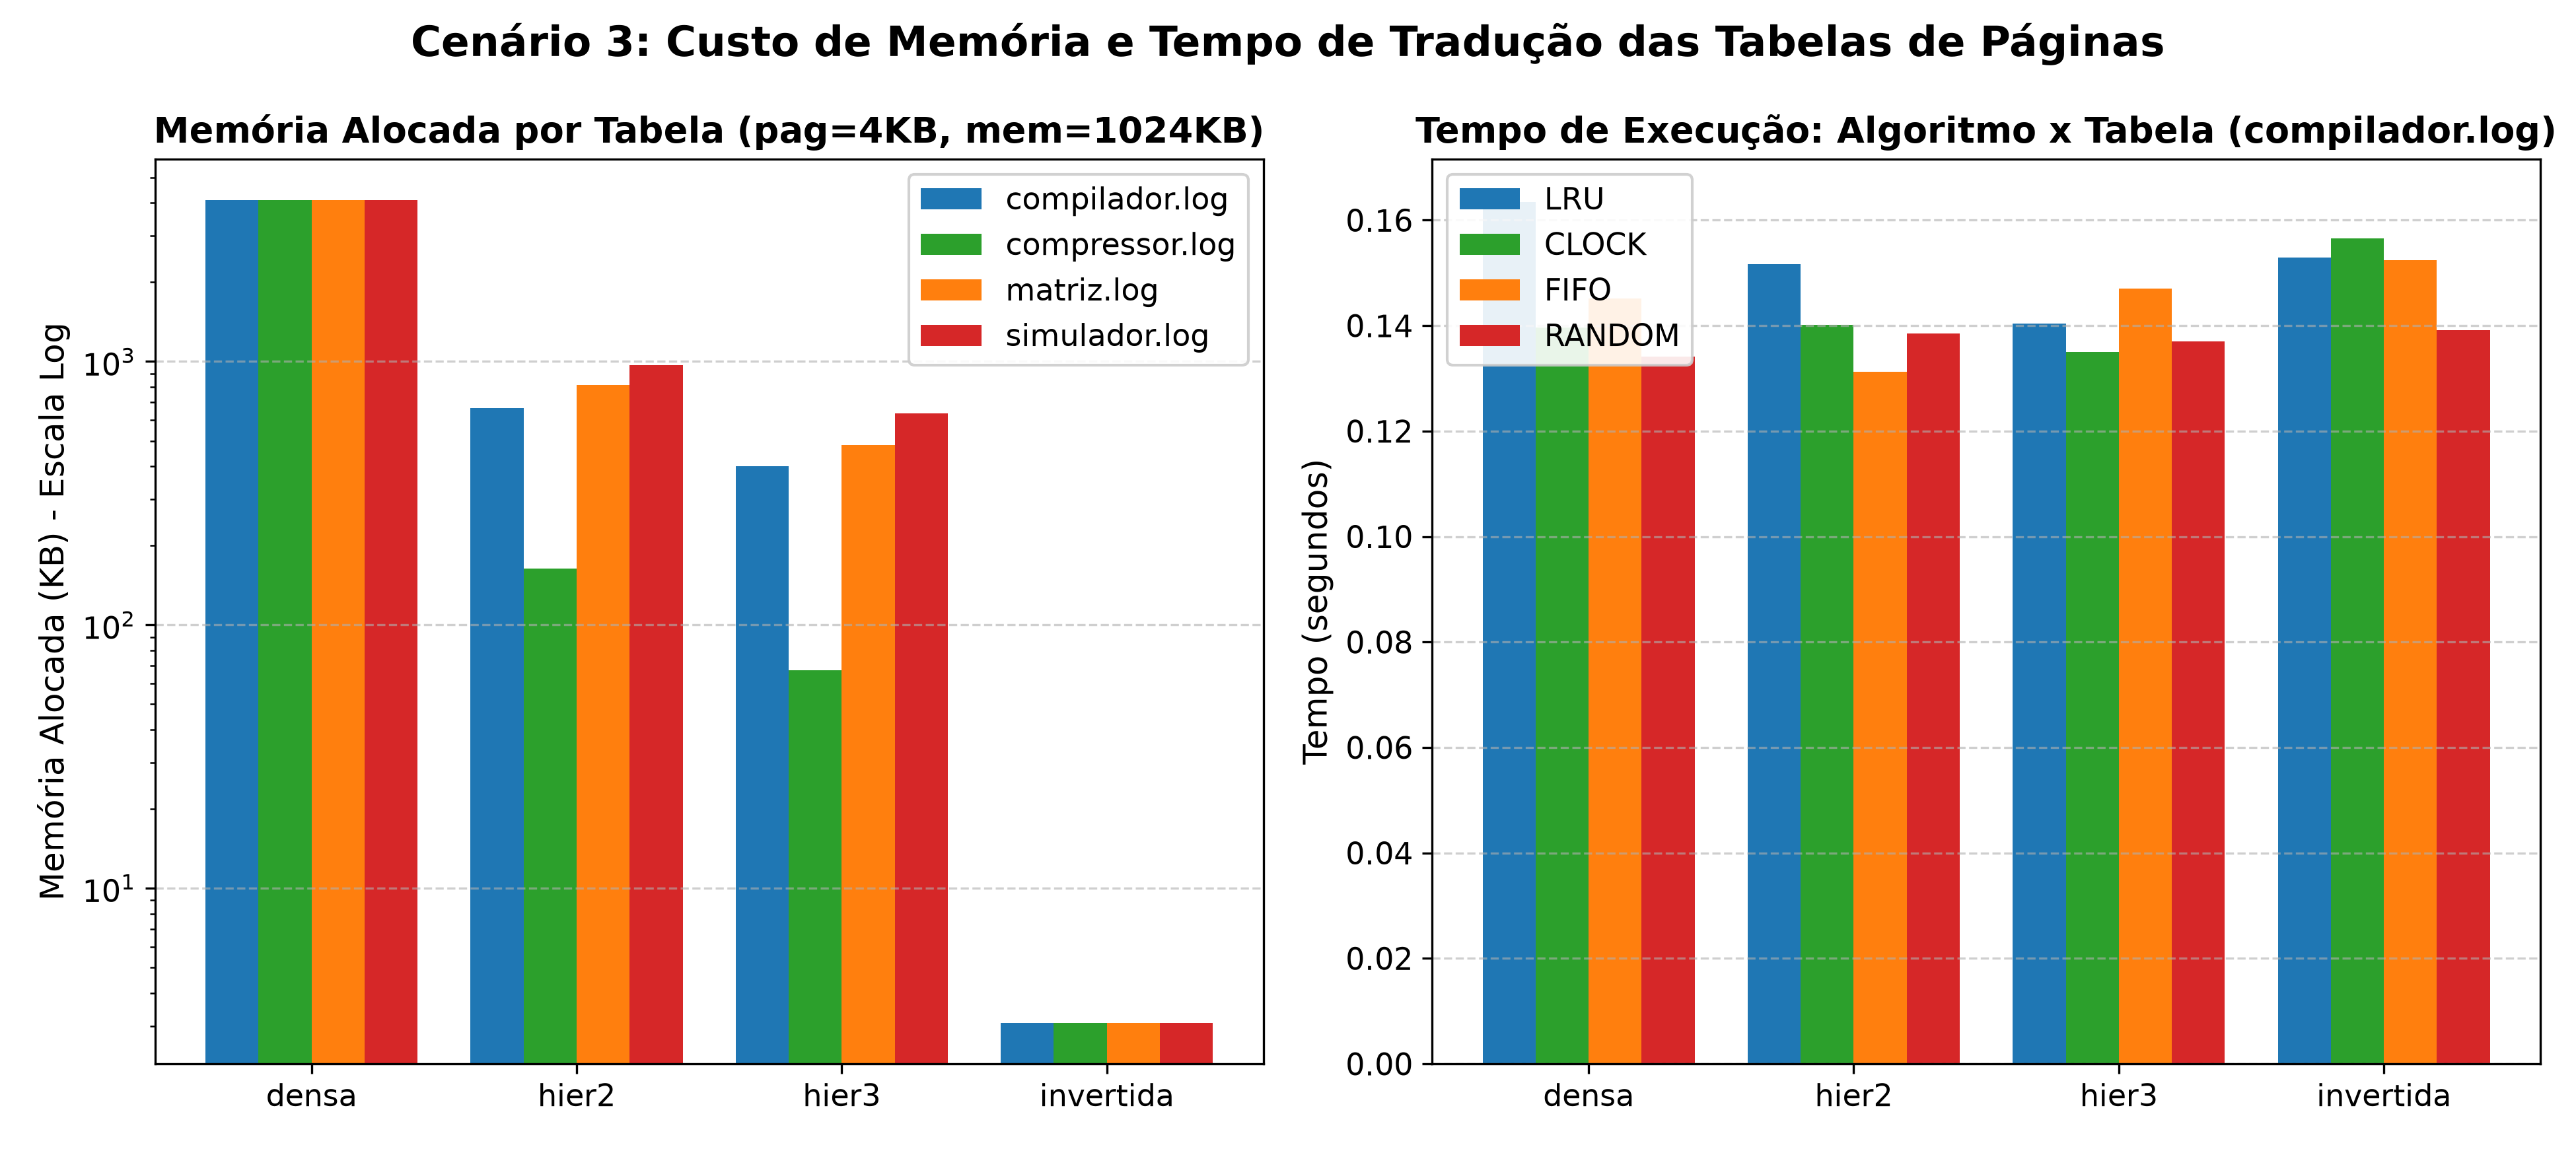
\includegraphics[width=1.0\textwidth]{results/cenario3_tabelas.png}
    \caption{Memória alocada nos 4 programas por tipo de tabela (esquerda) e tempo de execução cruzando cada algoritmo de substituição com as 4 tabelas (direita).}
    \label{fig:cenario3}
\end{figure}

Os resultados destacam três aspectos fundamentais:
\begin{itemize}
    \item \textbf{Tabela Densa vs. Tabelas Hierárquicas:} A tabela densa consome fixamente $4.194.392\text{ bytes}$ ($\approx 4\text{ MB}$), ou seja, $4\times$ mais memória que a própria RAM física simulada (1024 KB). Já as tabelas hierárquicas de 2 e 3 níveis alocam nós apenas para as regiões virtuais efetivamente tocadas: no \texttt{compressor.log} (espaço virtual compacto), a tabela de 2 níveis reduz o gasto para $168\text{ KB}$ ($-96\%$) e a de 3 níveis para $68,7\text{ KB}$ ($-98,4\%$). No \texttt{simulador.log}, cujos endereços são mais espalhados pelo espaço de 32 bits, mais sub-tabelas precisam ser instanciadas ($991\text{ KB}$ em 2 níveis e $652\text{ KB}$ em 3 níveis).
    \item \textbf{Eficiência espacial da Tabela Invertida:} A tabela invertida depende exclusivamente do número de quadros físicos ($256$ quadros em 1024 KB), consumindo exatamente \textbf{3.160 bytes ($\approx 3,1\text{ KB}$)} em qualquer programa --- uma redução de mais de \textbf{1.300 vezes} em relação à tabela densa. Quando a memória física é de 128 KB (32 quadros), seu consumo cai para apenas $472\text{ bytes}$.
    \item \textbf{Cruzamento Algoritmo $\times$ Tabela (Gráfico Direito da Figura~\ref{fig:cenario3}):} Comparar o LRU contra os demais algoritmos nas quatro tabelas mostra onde o tempo de CPU é gasto. Como a busca no LRU percorre os quadros ocupados ($O(Q)$ por falta) enquanto CLOCK, FIFO e Random têm decisão $O(1)$ amortizada, o LRU apresenta o maior tempo em todas as tabelas ($0,163\text{s}$ na densa contra $0,134\text{s}$ do Random). Além disso, passar da tabela densa/hierárquica para a invertida adiciona uma pequena sobrecarga devido ao caminhamento na lista de colisões do hash.
\end{itemize}

\subsection{Experimento Adicional 1: Investigação em Escala da Anomalia de Belady}

Para investigar a Anomalia de Belady de maneira sistemática (observando quantas vezes ela ocorre conforme aumentamos o tamanho da entrada e o número de quadros), construímos um gerador paramétrico de traces (\texttt{tests/trace\_belady\_N.log}, com $N \in \{500, 2.000, 10.000, 50.000\}$ acessos) que alterna fases cíclicas sobre janelas de $k \in \{5, 7, 9, 11, 13, 15\}$ páginas virtuais. Para cada tamanho de entrada $N$, executamos os algoritmos variando a memória passo a passo de $3$ até $32$ quadros físicos, contando quantas vezes a adição de um quadro físico extra ($Q \rightarrow Q+1$) provocou \textbf{aumento} no número de faltas de página. A Figura~\ref{fig:belady} e a Tabela~\ref{tab:belady} mostram os resultados.

\begin{figure}[H]
    \centering
    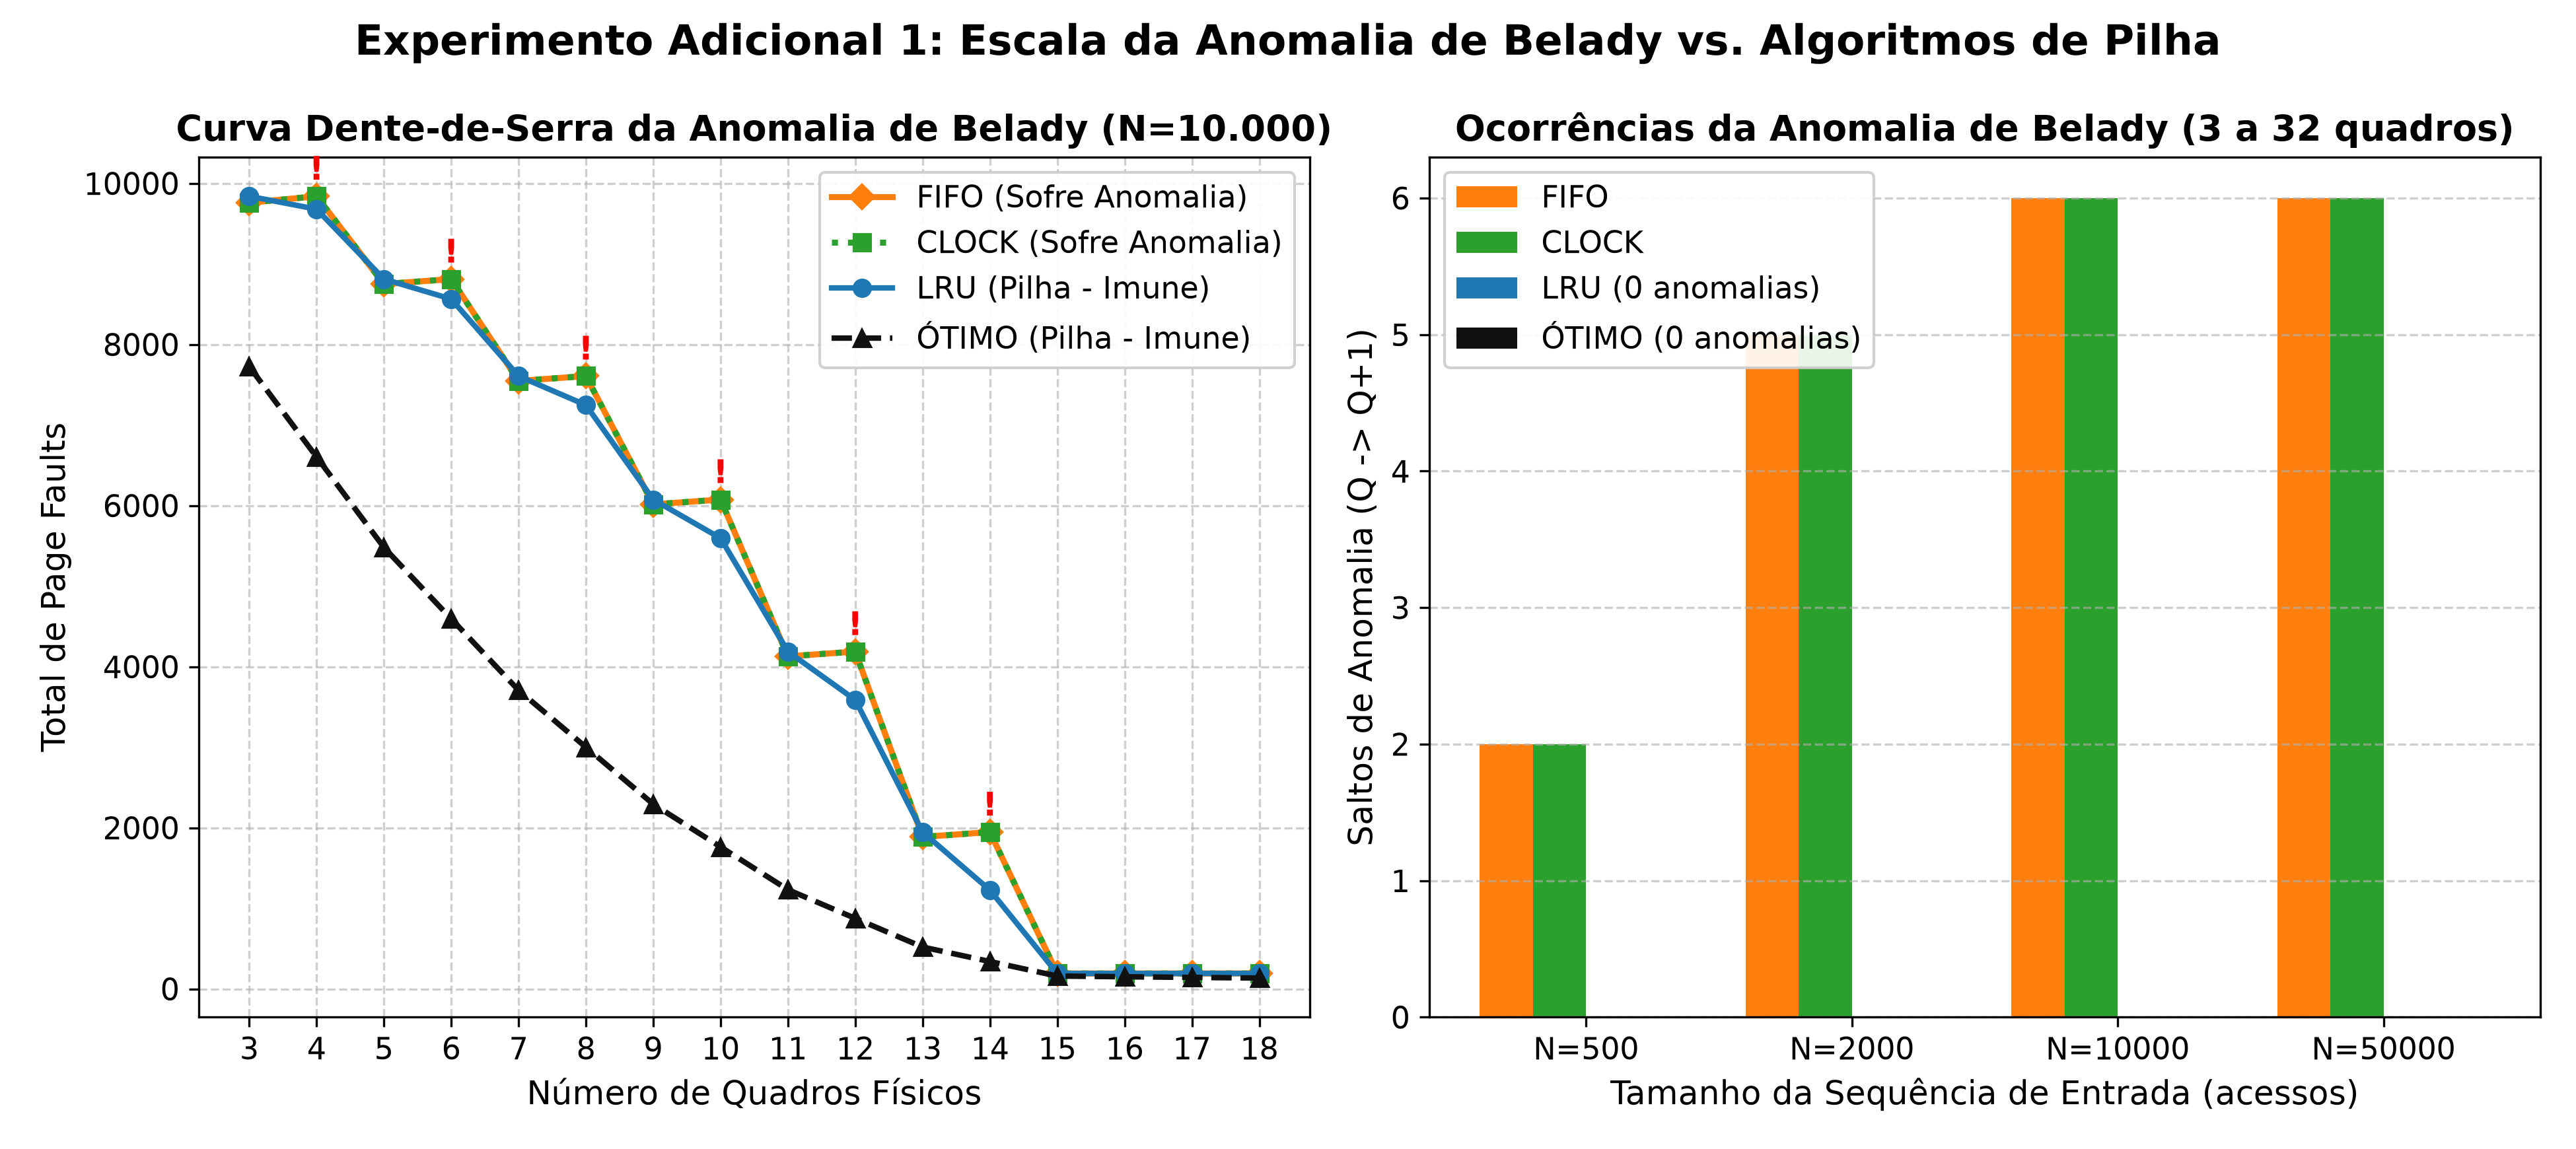
\includegraphics[width=1.0\textwidth]{results/cenario4_belady.png}
    \caption{Curva em dente-de-serra exibindo 6 saltos de Anomalia de Belady no FIFO e CLOCK para $N=10.000$ (esquerda) e contagem de ocorrências por tamanho de entrada (direita).}
    \label{fig:belady}
\end{figure}

\begin{table}[H]
\centering
\caption{Faltas de página em função do número de quadros ($N=10.000$ acessos), destacando em negrito os saltos onde ocorre a Anomalia de Belady ($Q \rightarrow Q+1$).}
\label{tab:belady}
\resizebox{\textwidth}{!}{%
\begin{tabular}{lrrrrrrrrrrrrr}
\toprule
\textbf{Algoritmo} & \textbf{3 q.} & \textbf{4 q.} & \textbf{5 q.} & \textbf{6 q.} & \textbf{7 q.} & \textbf{8 q.} & \textbf{9 q.} & \textbf{10 q.} & \textbf{11 q.} & \textbf{12 q.} & \textbf{13 q.} & \textbf{14 q.} & \textbf{15 q.} \\
\midrule
\textbf{FIFO}  & 9.760 & \textbf{9.840} & 8.750 & \textbf{8.812} & 7.548 & \textbf{7.608} & 6.015 & \textbf{6.075} & 4.128 & \textbf{4.188} & 1.887 & \textbf{1.947} & 192 \\
\textbf{CLOCK} & 9.760 & \textbf{9.840} & 8.750 & \textbf{8.812} & 7.548 & \textbf{7.608} & 6.015 & \textbf{6.075} & 4.128 & \textbf{4.188} & 1.887 & \textbf{1.947} & 192 \\
\textbf{LRU}   & 9.840 & 9.680          & 8.812 & 8.564          & 7.608 & 7.248          & 6.075 & 5.595          & 4.188 & 3.588          & 1.947 & 1.227          & 192 \\
\textbf{ÓTIMO} & 7.727 & 6.604          & 5.481 & 4.594          & 3.708 & 3.001          & 2.294 & 1.763          & 1.232 & 876            & 520   & 340            & 160 \\
\bottomrule
\end{tabular}%
}
\end{table}

Os resultados revelam comportamentos importantes:
\begin{enumerate}
    \item \textbf{Crescimento das ocorrências com a entrada e efeito dente-de-serra no FIFO e no CLOCK:} Conforme a sequência de entrada cresce de $N=500$ para $N=10.000$ e $50.000$ acessos (alcançando janelas cíclicas maiores), o número de transições $Q \rightarrow Q+1$ que sofrem a Anomalia de Belady sobe de $2$ para \textbf{6 episódios distintos} ($3\rightarrow4$, $5\rightarrow6$, $7\rightarrow8$, $9\rightarrow10$, $11\rightarrow12$ e $13\rightarrow14$ quadros). Mais interessante ainda é notar que o \textbf{CLOCK} sofre exatamente os mesmos saltos que o FIFO: quando as páginas da janela chegam sem reuso intermediário antes da substituição, todos os quadros estão com \texttt{ref == 1}, fazendo o ponteiro do relógio dar uma volta completa zerando os bits e degenerando exatamente na política FIFO.
    \item \textbf{Imunidade absoluta dos Algoritmos de Pilha (\textit{Stack Algorithms}):} Tanto o \textbf{LRU} quanto o \textbf{Ótimo} apresentaram \textbf{zero ocorrências} da anomalia em todos os tamanhos de trace ($N=500$ a $N=50.000$). Como ambos satisfazem a propriedade de inclusão de Mattson (o conjunto de páginas na memória com $Q$ quadros em qualquer instante é sempre um subconjunto estrito do conjunto com $Q+1$ quadros), suas curvas são estritamente decrescentes.
\end{enumerate}

\subsection{Experimento Adicional 2: Impacto do Dirty Bit}

Para investigar como o \textbf{LRU} e o \textbf{CLOCK} se comparam caso todas as páginas fossem sujas (isto é, se não existisse a verificação do \textit{dirty bit} e toda substituição após encher a memória exigisse escrita em disco: $\text{Escritas}_{\text{100\% dirty}} = \text{Faltas} - \text{Quadros}$), comparamos o volume de escritas nesse cenário contra as escritas reais filtradas pelo \textit{dirty bit}. A Figura~\ref{fig:dirty} ilustra essa análise.

\begin{figure}[H]
    \centering
    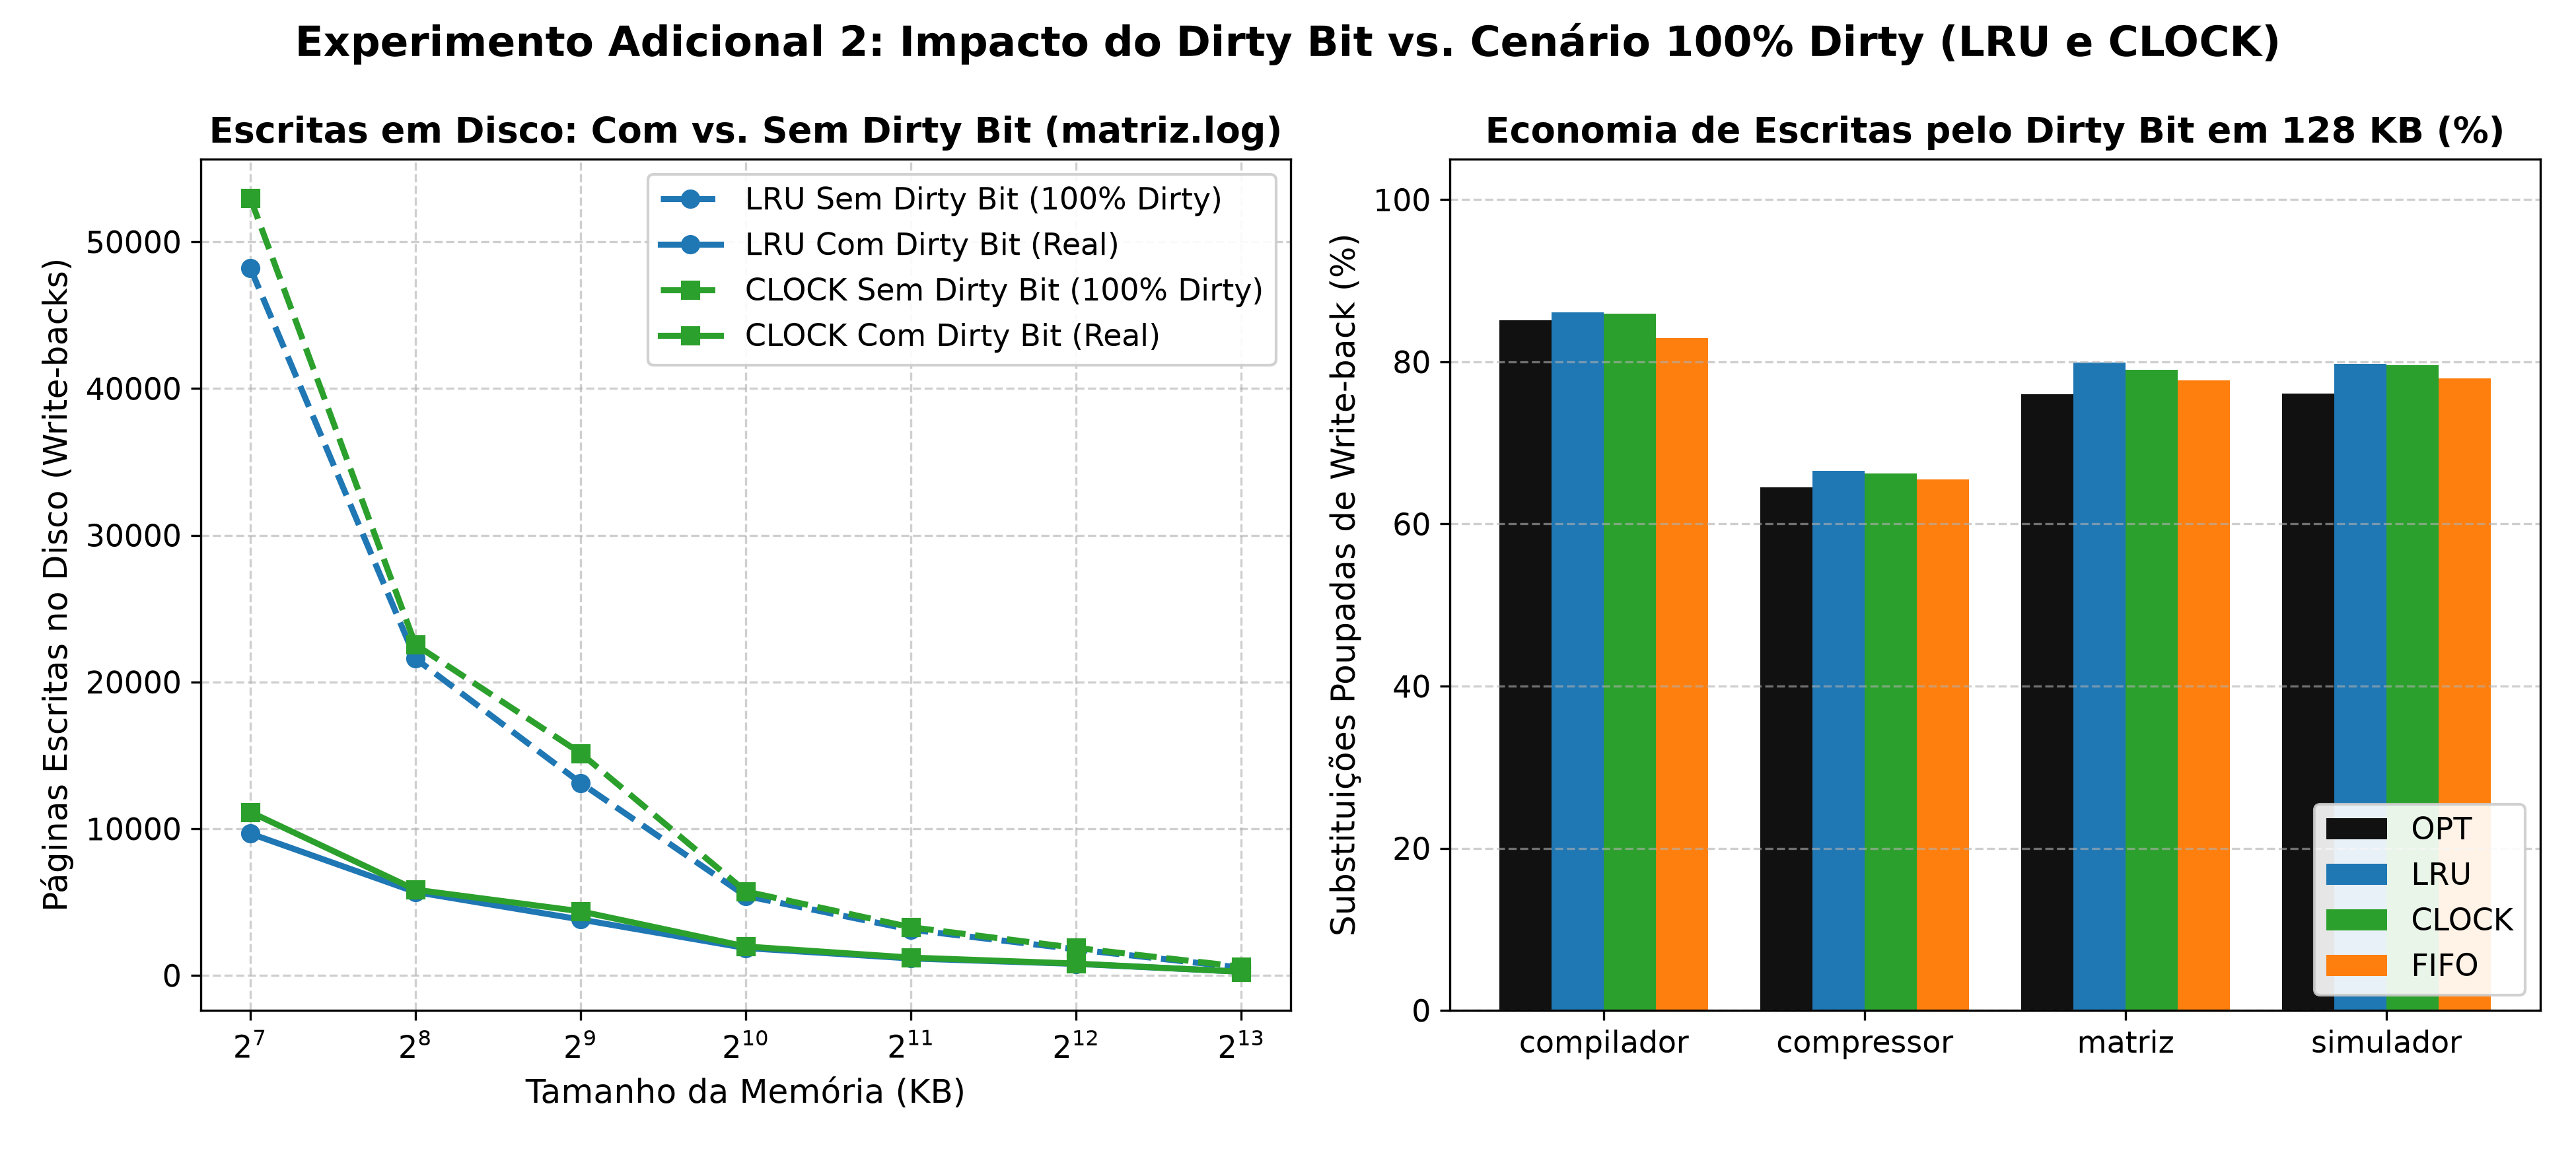
\includegraphics[width=1.0\textwidth]{results/cenario5_dirty_bit.png}
    \caption{Volume de escritas em disco em \texttt{matriz.log} com e sem verificação de \textit{dirty bit} (esquerda) e percentual de substituições poupadas de escrita em 128 KB (direita).}
    \label{fig:dirty}
\end{figure}

A análise mostra que:
\begin{enumerate}
    \item \textbf{Economia de escritas proporcionada pelo Dirty Bit:} Sem o bit de modificação (curvas tracejadas à esquerda na Figura~\ref{fig:dirty}), toda página desalojada em \texttt{matriz.log} (128 KB) precisaria ser copiada de volta ao disco, gerando $48.222$ escritas no LRU e $52.993$ no CLOCK. Com a verificação do \textit{dirty bit} (curvas cheias), as escritas caem para $9.674$ no LRU e $11.140$ no CLOCK --- uma \textbf{redução de $79,9\%$ e $79,0\%$ nas operações de escrita em disco}. No \texttt{compilador.log} (onde a maioria das páginas é de código ou tabelas apenas de leitura), a economia chega a \textbf{$86,1\%$}.
    \item \textbf{Comparação LRU vs. CLOCK com e sem Dirty Bit:} Se todas as páginas fossem tratadas como \textit{dirty}, o número de escritas em disco seria idêntico ao número de substituições ($\text{Faltas} - Q$), fazendo com que o CLOCK gerasse apenas $6,4\%$ mais escritas que o LRU no \texttt{compilador.log} e $9,9\%$ a mais no \texttt{matriz.log} (em 128 KB). Entretanto, quando o \textit{dirty bit} real está ativo em \texttt{matriz.log} (128 KB), a desvantagem do CLOCK nas escritas sobe para \textbf{$15,2\%$} ($11.140$ escritas no CLOCK contra $9.674$ no LRU). Isso ocorre porque páginas que sofrem escrita (como acumuladores e matrizes de saída) possuem altíssima localidade temporal: o LRU mantém essas páginas sujas protegidas no topo por mais tempo, enquanto a granularidade de 1 único bit do CLOCK ocasionalmente desaloja uma página suja após uma varredura do ponteiro, forçando sua escrita precoce em disco.
\end{enumerate}

\section{Conclusão}

Os experimentos realizados confirmaram as hipóteses teóricas sobre gerência de memória virtual e permitiram quantificar seus efeitos em traces reais e sintéticos. A inclusão do algoritmo \textbf{Ótimo de Belady (\texttt{opt})} estabeleceu o limite inferior de faltas de página em cada cenário, demonstrando que o \textbf{LRU} e o \textbf{CLOCK} operam muito próximos um do outro (diferença de apenas $3\%$ a $9\%$ em páginas lidas) e capturam a maior parte do ganho possível sobre políticas sem histórico de uso (\textbf{FIFO} e \textbf{Random}), que chegaram a gerar quase $70\%$ mais faltas e o dobro de escritas no trace \texttt{matriz.log}.

Nossos experimentos adicionais comprovaram em escala a diferença estrutural entre algoritmos de fila e algoritmos de pilha: enquanto o FIFO e o CLOCK exibiram até 6 episódios de Anomalia de Belady (curva em dente-de-serra) conforme o número de quadros cresceu de 3 para 32, o LRU e o Ótimo mantiveram monotonicidade estrita com zero anomalias. Além disso, a análise do \textit{dirty bit} revelou que a presença de 1 bit de modificação economiza entre $67\%$ e $86\%$ de todas as escritas em disco nos programas testados, e que o LRU protege páginas sujas melhor que o CLOCK simples (cuja diferença em relação ao LRU sobe de $9,9\%$ no cenário 100\% dirty para $15,2\%$ com o \textit{dirty bit} real em \texttt{matriz.log}).

Por fim, o estudo de variação do tamanho de página (2 KB a 64 KB) mostrou o colapso de desempenho (\textit{thrashing}) quando páginas excessivamente grandes reduzem o número de quadros físicos para apenas 16, e a avaliação das tabelas de páginas demonstrou a superioridade espacial das tabelas hierárquicas (economia de até $98,4\%$) e da tabela invertida com hash ($3,1\text{ KB}$ contra $4\text{ MB}$ da tabela densa). Como trabalho futuro, o algoritmo CLOCK pode ser estendido para a variante \textit{Enhanced Second-Chance} $\text{CLOCK}-(R,M)$, inspecionando o par $(\text{referência}, \text{modificação})$ para preferir vítimas limpas $(0,0)$ antes de desalojar páginas sujas $(0,1)$.

\end{document}
